\documentclass[hyperref={pdfpagelabels=false}]{beamer}

\usepackage[utf8]{inputenc}
\usepackage{lmodern}
\usepackage{amsmath}
\usepackage{amssymb}
% \usepackage{natbib}
\usepackage{verbatim}
\usepackage{floatpag}
\usepackage{subeqnarray}
\usepackage{mathrsfs}    %for special characters
\usepackage{cancel}  % to set terms in an equation to zero

\DeclareMathOperator*{\argmin}{arg\,min}

%Information to be included in the title page:
\title{Natural Gradient Method}
\author{Raghav K Singhal}
\institute{NYU Courant}
\date{2018}

\begin{document}
\frame{\titlepage}

\begin{frame}
\frametitle{Recap - Gradient Descent}
Gradient Descent tries to minimize a function $f(\theta)$ by taking steps of size $\alpha$ in the direction of the steepest descent,
\begin{align*}
\theta_{n+1} = \theta_{n} - \alpha \nabla_{\theta} f(\theta_{n})
\end{align*}
where $\nabla_{\theta} f(\theta_{n})$ is the direction of steepest descent:
\begin{align*}
\lim_{\epsilon \rightarrow 0} \argmin_{d\theta: || d\theta ||_2^2 \leq \epsilon^2 } f( \theta + d\theta) = \nabla_{\theta} f(\theta)
\end{align*}
\end{frame}

\begin{frame}
\frametitle{Problems with Euclidean Distance}

Let $p_{\theta} = \mathcal{N}(x | \mu, \sigma^2)$, where $\theta = [\mu, \sigma^2]$.
\\
Now for $\theta_1 = [0, 1000]^T$ and $\theta_2 = [10, 1000]^T$, the euclidean distance between $\theta_1, \theta_2$ is $10$, but they completely overlap.
\\
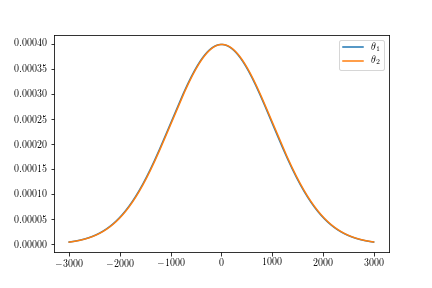
\includegraphics[scale=0.3]{experiment_1.png}
However, for $\theta_1 = [0, 0.01]^T$ and $\theta_2 = [0.1, 0.01]^T$, they barely overlap but the euclidean distance between them is $0.1$,
\\
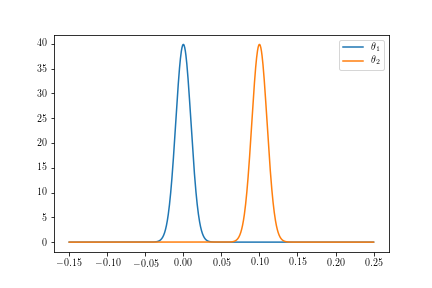
\includegraphics[scale=0.3]{experiment_2.png}
\end{frame}

\begin{frame}
\frametitle{Information Geometry}

The idea here is that in general the Euclidean metric is not the appropriate metric or distance function in parameter space.  \\
\
\\
We could use KL-divergence, but its not symmetric. However if we take a "local" view and analyze the geometry imposed by KL-Divergence, we realize that its  FAKE NEWS!
\end{frame}

\begin{frame}
\frametitle{KL Divergence}
\framesubtitle{A Really "CLOSE" look.}
We can show that KL-Divergence is 'locally' symmetric. Let $p_{\theta}$ be any smooth parametrized distribution. Now, we define the Fisher information matrix $G(\theta)$ as follows:
\begin{align*}
G(\theta) &= \mathbb{E}_{p_{\theta}}[\nabla_{\theta} \log p_{\theta}(x) \nabla_{\theta} \log p_{\theta}(x)^T] \\
&= -\mathbb{E}_{p_{\theta}}[\nabla^{2}_{\theta} \log p_{\theta}]
\end{align*}
Then note that by taking a Taylor Series expansian around $\theta$
\begin{align*}
\text{KL}(p_{\theta + d\theta}(x) || p_{\theta}(x)) = \frac{1}{2} d\theta^T G(\theta) d\theta + \mathcal{O}(||d\theta||^3) \\
\text{KL}(p_{\theta}(x) || p_{\theta + d\theta}(x)) = \frac{1}{2} d\theta^T G(\theta) d\theta + \mathcal{O}(||d\theta||^3)
\end{align*}

Therefore, $\text{KL}(p_{\theta + d\theta}(x) || p_{\theta}(x)) = \text{KL}(p_{\theta}(x) || p_{\theta + d\theta}(x))$. Hence, KL-Divergence is locally symmetric.
\end{frame}

\begin{frame}
\frametitle{Natural Gradients}
Now, the directioin of steepest descent in this geometry, induced by the Fisher metric, is as follows:
\begin{align*}
\lim_{\epsilon \rightarrow 0} \argmin_{d\theta: KL(\theta || \theta + d\theta) \leq \epsilon } f( \theta + d\theta) = G(\theta)^{-1} \nabla_{\theta} f(\theta)
\end{align*}
where we define $G(\theta)^{-1} \nabla_{\theta} f(\theta)$ as the natural gradient $\tilde{\nabla}_{\theta} f(\theta)$. \\
\
\\
 So gradient descent in this space is as follows:
\begin{align*}
\theta_{n+1} &= \theta_{n} - \alpha \tilde{\nabla}_{\theta} f(\theta_n) \\
&= \theta_{n} - \alpha G(\theta)^{-1} \nabla_{\theta} f(\theta_n)
\end{align*}
\end{frame}

\begin{frame}
\frametitle{Information Geometry}
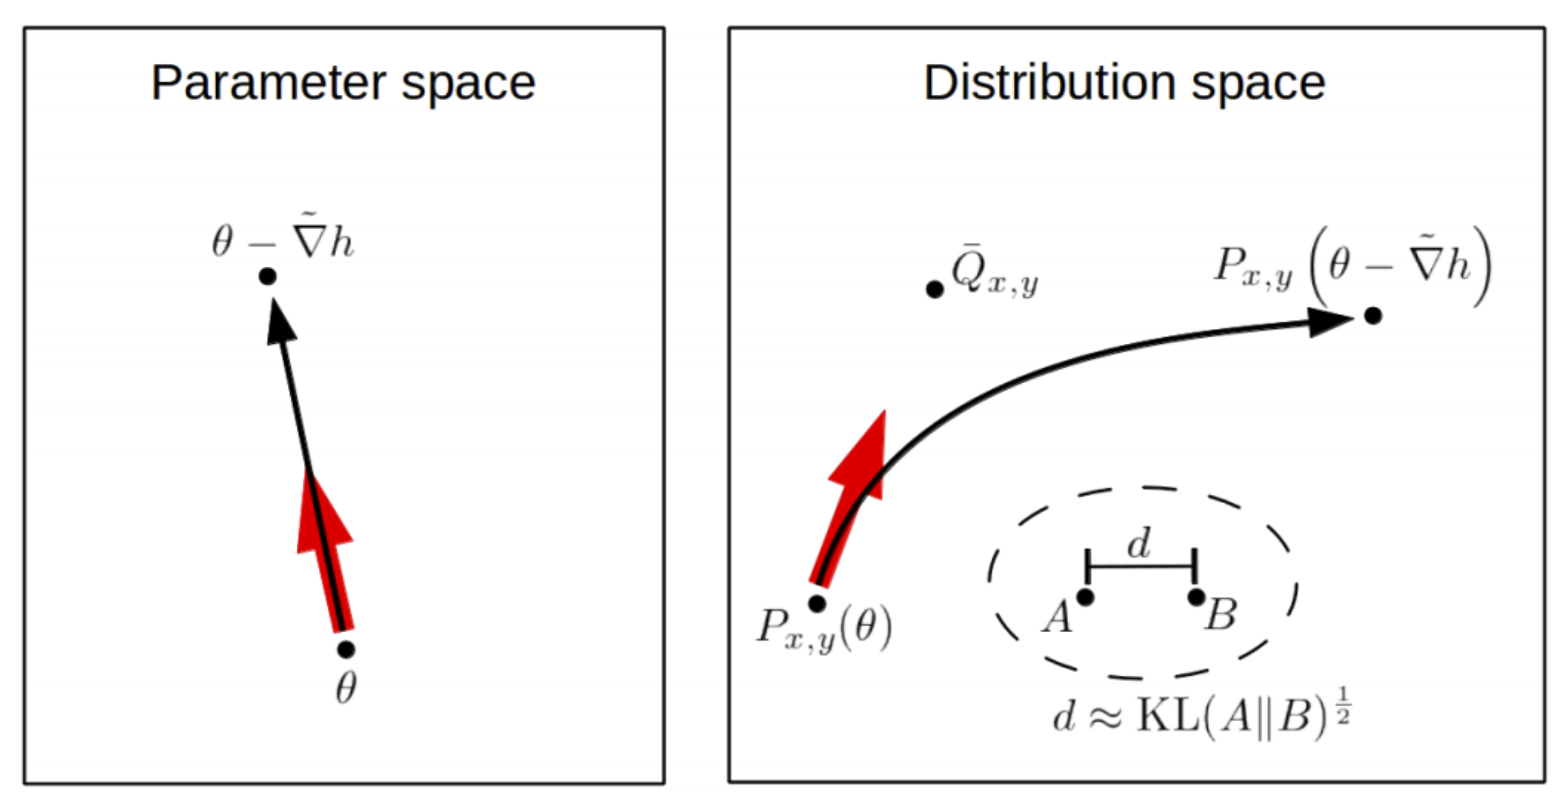
\includegraphics[scale=0.3]{ng.png}
 The red arrow is the natural gradient direction, given by the vector $G(\theta)^{-1}\nabla h(\theta)$ in parameter space and the black arrow is the path generated by taking $\theta - \alpha G(\theta)^{-1}\nabla h$.
\end{frame}


\begin{frame}
\frametitle{The Fisher}
This formulation induces a Riemannian Geometry and we can view the Fisher matrix as inducing a norm in the distribution space:
\begin{align*}
|| p_{\theta}||_{G_{\theta}} = \left\langle p_{\theta}, G(\theta) p_{\theta} \right\rangle
\end{align*}
so this naturally gives us notions of length, geodesics, etc.\\
\
\\
 A geodesic is the shortest path between two points, for example in a Euclidean Space, the shortest distance between two points is a straight line, however in Riemannian Manifolds, the shortest distance between two points can be curved and is not unique.
\end{frame}


\begin{frame}
\frametitle{Properties of Natural Gradients}
\begin{enumerate}
\item We have now formulated the gradient descent algorithm in the space of prediction functions or distributions rather than parameters

\item When the natural gradient descent algorithm approches the optimum, i.e. $\mathbb{P}_{\theta}$ approches $\mathbb{Q}$, the Fisher matrix $G(\theta)$ approaches the true hessian of the loss function, $\mathbb{E}_{\mathbb{Q}}[\nabla^{2} f(\theta)]$.

% \begin{align*}
% \end{align*}∫

\item However, getting the actual Fisher Matrix is infeasible in most settings. So some authors suggest using the following approximation:

\begin{align*}
\tilde{G}(\theta) = \frac{1}{n}\sum_{i=1}^{n} \nabla_{\theta}p_{\theta}(x_i) \nabla_{\theta}p_{\theta}(x_i)^T
\end{align*}
Note that this approximation is different from our previous formulation, as $\tilde{G}(\theta) = \mathbb{E}_{\hat{\mathbb{Q}}} [\nabla_{\theta}p_{\theta}(x) \nabla_{\theta}p_{\theta}(x)^T]$.
\end{enumerate}
\end{frame}

% \begin{frame}
% \frametitle{There Is No Largest Prime Number}
% \framesubtitle{The proof uses \textit{reductio ad absurdum}.}
% \begin{theorem}
% There is no largest prime number.
% \end{theorem}
% \begin{proof}
% \begin{enumerate}
% \item<1-| alert@1> Suppose $p$ were the largest prime number.
% % \item<2-> Let $q$ be the product of the first $p$ numbers.
% % \item<3-> Then $q+1$ is not divisible by any of them.
% % \item<1-> But $q + 1$ is greater than $1$, thus divisible by some prime
% % number not in the first $p$ numbers.\qedhere
% \end{enumerate}
% \end{proof}
% \end{frame}


\end{document}
